\section{Technical overview}
\label{sec:tech-overview}

In the related work section, we surveyed two approaches to the model checking problem in previous results.
Our algorithm combines ideas from both approaches:
\begin{itemize}
  \item[--] decomposition-based methods, to do dynamic programming along a construction sequence with almost bounded merge-width; and
  \item[--]  stability-theoretic bounds on the \emph{number of types}, allowing us to bound the runtime of the algorithm.
\end{itemize}
In this section, we give a high-level overview of the algorithm and the interplay between the two components.
We start by introducing the relevant definition.

\paragraph{Merge-width.}
The merge-width parameters are defined through decompositions called \emph{construction sequences}~\cite{mw-stoc}.
We can define them as follows.
% lax begin Lax185574.PartialGraphs
\begin{itemize}%
    \item A \emph{partial graph} $H$ consists of a finite vertex set $V=V(H)$, two disjoint sets $E(H),N(H)\subseteq\binom V2$ of \emph{edges} and \emph{non-edges}, and a partition of $V$ whose parts we treat as colors.
    The pairs in $R(H)\coloneqq E(H)\cup N(H)$ are \emph{resolved}, and all other pairs are \emph{unresolved}.
    We view $H$ as a logical structure with binary relations $E$ and $N$ and a unary predicate for every color.
    Distances $\dist^H$ and balls $\Ball^H_r(v)$ are measured in the Gaifman graph $(V,R(H))$, the graph of resolved pairs.
% lax end
% lax begin Lax185574.ConstructionSequences
    \item For two distinct parts $P,Q$ of $H$, the \emph{merge} of $P$ and $Q$ replaces them by the single part $P\cup Q$.
    For two parts $P,Q$ of $H$ (possibly $P=Q$), the \emph{positive resolve} of $P$ and $Q$ adds all unresolved pairs $uv$ with $u\in P$ and $v\in Q$ to $E(H)$, while the \emph{negative resolve} adds them to $N(H)$.
    \item A \emph{construction sequence} of a graph $G=(V,E)$ is a sequence $G_1,\ldots,G_\lambda$ of partial graphs with vertex set $V$,
    such that $G_1$ has no resolved pairs and only singleton parts, every $G_{t+1}$ is obtained from $G_t$ by one merge or one resolve,
    and, finally, $G_\lambda$ has a single part, $E(G_\lambda)=E$, and $N(G_\lambda)=\binom V2\setminus E$.
% lax end
% lax begin Lax185574.ConstructionWidth
    \item The \emph{radius-$r$ width} of the sequence is the maximum, over all $t\in[\lambda]$ and $v\in V$, of the number of parts of $G_t$ that intersect $\Ball^{G_t}_r(v)$.
    The \emph{radius-$r$ merge-width} of $G$ is the minimum radius-$r$ width over all construction sequences of $G$.
% lax end
\end{itemize}

% lax begin Lax185574Proofs.ChainTheorem.exists_program_decreasingChain
In a companion paper, together with Micha\l{} Pilipczuk, we prove that monadically dependent classes have \emph{almost bounded merge-width}~\cite{md-abmw}, and that witnessing construction sequences can be computed efficiently.
% lax end
These construction sequences form the backbone of our model checking algorithm.

\begin{theorem}[\cite{md-abmw}]\label{thm:ov-abmw}
  Let $\CC$ be a monadically dependent graph class and $r\in\N$.
  Every $n$-vertex graph $G\in\CC$ has radius-$r$ merge-width $n^{o(1)}$, and a witnessing construction sequence can be computed in time $O_{\CC,r}(n^{3+o(1)})$.
\end{theorem}

\paragraph{Types along decompositions.}
Many model checking algorithms (including ours) process a decomposition of the input graph step by step, and maintain \emph{types}: formulas of bounded quantifier rank satisfied by the intermediate graphs processed so far.
For example, Courcelle's theorem~\cite{courcelle1990monadic} maintains, for every node $t$ of a tree decomposition with bag $\tup b=(b_1,\ldots,b_k)$, the type
\[
\setof{\psi(x_1,\ldots,x_k)}{\text{$\psi$ is an MSO formula of quantifier rank at most $q$, such that $\psi(\tup b)$ holds in $G_t$}},
\]
where $G_t$ is the subgraph induced by the bags in the subtree of $t$. Here $q$ is the quantifier rank of the input formula $\phi$.
The type above is computed from the types of the children of $t$.
Similarly, the algorithms for bounded twin-width maintain FO types along contraction sequences~\cite{tww1,tww-types-icalp}, and the algorithm for bounded merge-width along construction sequences~\cite{mw-arxiv}.

We call a first-order formula \emph{local} if, roughly speaking, every quantifier has the form
\begin{center}
  $\exists y\,(\dist(\tup x,y)\le r\land\chi(\tup x y))$ \quad or \quad $\forall y\,(\dist(\tup x,y)\le r\to\chi(\tup x y))$
\end{center}
ranging only over vertices close to some free or previously quantified variables $\tup x$.
The merge-width model checking algorithm~\cite{mw-arxiv} maintains, at every step $H$ of the construction sequence and for every vertex $v$, its \emph{local type} of quantifier rank $q$, for some constant $q$ depending on $\phi$:
\[
\setof{\psi(x)}{\text{$\psi$ is a local formula of quantifier rank at most $q$, such that $\psi(v)$ holds in $H$}}.
\]
In the first step of the construction sequence, nothing is resolved, and the local types are trivial.
In the last step, all pairs are resolved, and the local types determine whether the input sentence $\phi$ holds in $G$.
In between, the local types have to be updated after every merge and every resolve.
Merges are handled easily, by simply rewriting color names; the main difficulty in~\cite{mw-arxiv} is to lift the local types through resolves.

\paragraph{Combinatorial explosion.}
For all these type-based model checking algorithms, the number of possible types grows non-elementarily with the width of the decomposition.
In particular, in each step of a construction sequence of radius-$r$ width $w$, each vertex locally reaches at most $w$ colors, and the number of local formulas over $w$ colors is a tower of exponentials in $w$.
This is a constant if the width \(w\) is treated as a constant (the radius $r$ here is fixed and depends on the quantifier rank $q$).
However, monadically dependent classes may have unbounded merge-width, and we can only guarantee a merge-width bound of \(w = n^{o(1)}\).
In this case the number of all possible local types explodes.

\paragraph{Our algorithm.}
The tower above counts the types that are \emph{possible} with $w$ colors.
Our starting point is the observation that in monadically dependent classes, only few of them are \emph{realized}, that is, actually occur as the type of some tuple of vertices of the input graph.
We keep the overall structure of the merge-width algorithm, but change it so that its running time depends only on the realized types.
This has three parts, which we describe in the rest of this section.
\begin{enumerate}
  \item We represent local types by \emph{type trees}, whose size depends only on the realized types.
  \item We show that only $n^{o(1)}$ types are realized in a ball, which bounds the size of type trees (\Cref{lem:ov-tree-size}).
  \item We lift type trees through merges and resolves in time polynomial in $n$ and the number of realized types (\Cref{lem:ov-resolve-lift}).
\end{enumerate}

\paragraph{Type trees.}
Type trees (defined in \Cref{sec:typetrees}) are a variant of Hintikka types~\cite{Scott1979}.
Simplifying for the sake of presentation, up to the precise choice of radii $r_1<r_2<\ldots$, the type tree of a tuple $\tup a$ is
\[
\tree_q(\tup a)\coloneqq
\begin{cases}
\atp(\tup a)&\text{if $q=0$,}\\
\bigl(\atp(\tup a),\ \setof{(i,\tree_{q-1}(\tup a b))}{i\in[|\tup a|],\ b\in V,\ \dist(a_i,b)\le r_q}\bigr)&\text{if $q>0$,}
\end{cases}
\]
where $\atp(\tup a)$ is the set of atomic formulas satisfied by $\tup a$, including atoms that compare distances between the entries of $\tup a$ and the colors.
The index $i$ records which entry of $\tup a$ is close to $b$.
Two tuples have the same type tree if and only if they have the same local type (\Cref{cor:tp-tree}), so type trees are just another representation of local types.
Type trees resemble the morphism-trees of~\cite{tww1} and serve a similar purpose.
\Cref{fig:ov-type-tree} shows an example.

\begin{center}
  \begin{tikzpicture}[
      vx/.style={circle, fill, inner sep=1.6pt},
      vy/.style={circle, fill=blue!65!black, inner sep=1.4pt},
      vz/.style={rectangle, fill=orange!85!black, inner sep=1.8pt},
      e/.style={gray!70!black},
      tnode/.style={draw, rounded corners=2pt, font=\scriptsize, align=center, inner sep=3pt, fill=white},
      tedge/.style={gray!70!black},
      lbl/.style={font=\scriptsize},
      ilbl/.style={font=\scriptsize, inner sep=1pt}
    ]
    \fill[gray!10] (0,0) circle (1.4);
    \draw[gray, dashed] (0,0) circle (1.4);
    \node[lbl, gray!60!black] at (135:1.85) {$\Ball_{r_1}(a)$};
    \node[vx] (a) at (0,0) {};
    \node[lbl] at (270:0.3) {$a$};
    \foreach \ang/\v in {90/b,162/c,234/d} {
      \node[vy] (\v) at (\ang:0.95) {};
      \node[lbl] at (\ang:1.2) {$\v$};
      \draw[e] (a) -- (\v);
    }
    \foreach \ang/\v in {306/e,18/f} {
      \node[vz] (\v) at (\ang:0.95) {};
      \draw[e] (a) -- (\v);
    }
    \node[lbl] at (306:1.2) {$e$};
    \node[lbl, above=2pt of f] {$f$};
    \node[vy] (g) at (2.2,0.75) {};
    \node[lbl, right=2pt of g] {$g$};
    \draw[e] (f) -- (g);
    \node[vx] at (-0.9,-1.95) {};
    \node[lbl, right] at (-0.85,-1.95) {$X$};
    \node[vy] at (-0.05,-1.95) {};
    \node[lbl, right, text=blue!65!black] at (0,-1.95) {$Y$};
    \node[vz] at (0.8,-1.95) {};
    \node[lbl, right, text=orange!85!black] at (0.85,-1.95) {$Z$};
    \begin{scope}[yshift=-0.65cm]
      \node[tnode] (root) at (6.3,1.35) {$X(x_1)$};
      \node[lbl, left=6pt of root] {$\tree_1(a)$};
      \node[tnode] (c1) at (4.0,-0.55) {$x_1=x_2$\\ $X(x_2)$};
      \node[tnode] (c2) at (6.3,-0.55) {$x_1\neq x_2$\\$E(x_1,x_2)$\\ \textcolor{blue!65!black}{$Y(x_2)$}};
      \node[tnode] (c3) at (8.6,-0.55) {$x_1\neq x_2$\\$E(x_1,x_2)$\\ \textcolor{orange!85!black}{$Z(x_2)$}};
      \draw[tedge] (root) -- node[ilbl, pos=0.38,
      above=1pt] {$1$} (c1);
      \draw[tedge] (root) -- node[ilbl, pos=0.38,
      left=1pt] {$1$} (c2);
      \draw[tedge] (root) -- node[ilbl, pos=0.38,
      above=1pt] {$1$} (c3);
      \node[ilbl, below=4pt of c1] {$a$};
      \node[ilbl, below=4pt of c2, text=blue!65!black] {$b,c,d$};
      \node[ilbl, below=4pt of c3, text=orange!85!black] {$e,f$};
    \end{scope}
  \end{tikzpicture}
  \captionof{figure}{\emph{Left:} A partial graph with $7$ vertices and colors $X,Y,Z$. \emph{Right:} $\tree_q(a)$ for $q=1$ and $r_1=1$, drawn as a tree of depth $q$ whose nodes are the sets $\atp(a)$ and $\atp(a\,v)$. The edge label $1$ records that $v$ is close to the first entry of the tuple $(a)$. The lists of vertex labels below the boxes show which vertices of $\Ball_{r_1}(a)$ give each child of the root node. The vertex $g$ outside the locality radius \(r_1 = 1\) does not occur in the tree. Note that the size of the tree adapts to the number of atomic types $\atp(a\,v)$ realized in the ball.}
  \label{fig:ov-type-tree}
\end{center}

Type trees carry the same information as local types, but they may have a much smaller representation.
The type tree of a tuple $\tup a$ has one subtree for every type tree realized by an extension $\tup a b$ with $b$ close to some component $a_i$ of $\tup a$, so its size is governed by the nearby realized types rather than by the possible ones.
Roughly, this is like storing a small subset of a huge universe as the list of its elements, whereas naive type-based algorithms store it as its characteristic vector.
Showing that type trees have size $n^{o(1)}$ is a key step of our algorithm.
For this, we first leave the algorithm aside for a moment.

\paragraph{Counting types over parameters.}
We turn to a purely quantitative result about monadically dependent classes, which counts types over a set of parameters and may be of independent interest.
Let $H$ be a graph or partial graph, $U\subseteq V(H)$, and $k,q\in\N$.
The \emph{type over $U$} of a tuple $\tup a\in V(H)^k$ is the set of first-order formulas $\psi(x_1,\ldots,x_k)$ of quantifier rank at most $q$ which are satisfied by $\tup a$ in $H$,
where $\psi$ may use any number of vertices of $U$ as constants, called \emph{parameters}. We denote this type by $\tp^H_q(\tup a/U)$.
For $X\subseteq V(H)$, we write $\Types^H_{k,q}(X/U)$ for the set of types over $U$ of tuples from $X^k$,
$$\Types^H_{k,q}(X/U)=\setof{\tp^H_q(\tup a/U)}{\tup a\in X^k}.$$
This set has at most $|X|^k$ elements, but can be much smaller, as two tuples  have the same type if no formula distinguishes them.
We write $\Types^H_{k,q}(X)$ if $U=\emptyset$.
One of the main contributions of this paper is the following bound on the number of types over parameters in monadically dependent graph classes.

% lax begin Lax185574.TypeBound
\begin{theorem}[Simplified form of \Cref{thm:type-bound}]\label{thm:ov-type-bound}
  Let $\CC$ be a monadically dependent graph class and $k,q\in\N$. There is some $d\in\N$ such that for every $G\in\CC$ and every set $U\subseteq V(G)$ with $|U|>1$,
  $$|\Types^G_{k,q}(V(G)/U)|\le |U|^d.$$
\end{theorem}
% lax end

The proof of \Cref{thm:ov-type-bound} proceeds as follows. We fix some radius $r$ depending on the quantifier rank $q$.
We then show (in \Cref{thm:closures})  that there is a set $\wh U$ of size polynomial in $|U|$,
such that for every vertex $v\in V(G)$,
there is some  \emph{separator} $S\subseteq \wh U$ of size bounded by some constant $s$,
such that $S$ \emph{separates} $v$ from $U$ \emph{at a distance} $r$.
The notion of separation is technical,
but it ensures that the following holds
for all $v\in V(G)$ which are $r$-separated from $U$ by $S$:
\begin{quote}\centering
The type $\tp^G_q(v/U)$ is determined by the type $\tp^G_{q'}(v/S)$.
\end{quote}
Here $q'$ depends only on $q$.
Since $S$ has size bounded by $s$, and both $s$ and $q'$ are constants (depending only on $\CC$ and $q$),
the number of types $\tp^G_{q'}(v/S)$ is bounded by a constant $c$ (depending on $\CC$ and $q$). Since there are at most $|\wh U|^s$ considered separators $S$, it follows that altogether there are at most $c\cdot |\wh U|^s$  types over $U$ of single vertices $v\in V(G)$, of quantifier rank $q$. This gives the required polynomial bound on the number of types of single vertices $v$ over a set~$U$. The argument for $k$-tuples $\tup v$ proceeds similarly.

\paragraph{The size of type trees.}
We now return to type trees and bound their sizes using the bound on the number of types.
The following lemma makes precise that type trees store only the types realized nearby.

% lax begin Lax185574.TypeTreeSizes
\begin{lemma}[informal version of \Cref{lem:ball-tree-bound}]\label{lem:ov-tree-size}
  Let $q\in\N$. There is $d\in\N$ depending only on $q$ such that for every partial graph $H$ and vertex $v$,
  the type tree $\tree_q(v)$ in $H$ has size polynomial in $K\coloneqq|\Types^H_{d,d}(\Ball^H_d(v))|$.
\end{lemma}
% lax end

We bound $K$ in \Cref{lem:ov-tree-size} using the bound on the number of types (\Cref{thm:ov-type-bound}).
The two count different things.
$K$ counts types without parameters in a partial graph $G_t$, whose colors are not present in $G$, and resolved pairs a priori form an arbitrary subset of vertex pairs.
On the other hand, the type bound counts types in $G$ itself, over a set of parameters.
While \(G\) comes from a monadically dependent graph class, \(G_t\) a priori does not, making it difficult to enforce structural properties on \(G_t\).

We bridge this gap by computing construction sequences that are \emph{locally definable} in $G$:
in every local ball, the colors and resolved pairs of $G_t$ can be expressed by first-order formulas in $G$ that mention only $n^{o(1)}$ vertices as parameters.
A challenge in encoding $G_t$ into $G$ is that $G_t$ accumulates many resolves over time, which cannot be modeled nicely by parameters.
To overcome this, we turn to \emph{merge sequences}, which group many merges and resolves into a single step, and can therefore be much shorter than construction sequences.
For every $\eps>0$,~\cite{md-abmw} provides a chain of sets $V(G)=S_1\supseteq\dots\supseteq S_\ell=\emptyset$, a closely related decomposition, with only $\ell=O(1/\eps)$ steps, which we convert into a merge sequence of width $n^{O(\eps)}$ with the same number of steps.
Each step can be encoded in $G$ by $O(1)$ unary predicates, and when we refine the merge sequence into a construction sequence, every $G_t$ stays locally definable using these $O(1/\eps)$ predicates and few parameters.
The bound on the number of types (\Cref{thm:ov-type-bound}) extends to such expansions of $G$ by boundedly many unary predicates, so it bounds $K$ by $n^{O(\eps)}$, and by \Cref{lem:ov-tree-size}, every type tree has size $n^{O(\eps)}$ as well.

\paragraph{Lifting type trees through merges and resolves.}
Now that we know that type trees are small, it remains to compute them efficiently.
Our algorithm processes the construction sequence step by step and maintains the type tree of every vertex.
So after every merge and every resolve, it has to compute the new type trees from the old ones.
Merges are easy.
Merging two parts $P$ and $Q$ into $P\cup Q$ does not change the resolved pairs, and hence not the distances.
Given a type tree from before the merge, we can update it as follows:
in every node, remove all atoms that mention $P$ or $Q$, and add an atom mentioning $P\cup Q$ whenever the same atom with $P$ or with $Q$ in its place was present.
The difficulty lies in resolves, which create new short paths and thereby bring new vertices close to a vertex $v$ (see \Cref{fig:ov-resolve}).

\begin{center}
  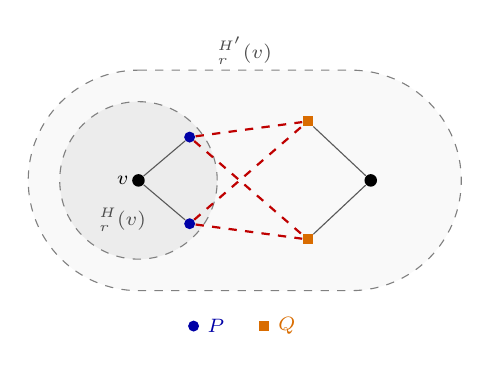
\begin{tikzpicture}[
      vx/.style={circle, fill, inner sep=1.6pt},
      vp/.style={circle, fill=blue!65!black, inner sep=1.4pt},
      vq/.style={rectangle, fill=orange!85!black, inner sep=1.8pt},
      e/.style={gray!70!black},
      new/.style={red!75!black, thick, dashed},
      lbl/.style={font=\scriptsize}
    ]
    \fill[gray!5] (0,1.4) -- (2.7,1.4) arc[start angle=90, end angle=-90, radius=1.4] -- (0,-1.4) arc[start angle=270, end angle=90, radius=1.4] -- cycle;
    \draw[gray, dashed] (0,1.4) -- (2.7,1.4) arc[start angle=90, end angle=-90, radius=1.4] -- (0,-1.4) arc[start angle=270, end angle=90, radius=1.4] -- cycle;
    \node[lbl, gray!60!black] at (1.35,1.65) {$\Ball^{H'}_r(v)$};
    \fill[gray!15] (0,0) circle (1);
    \draw[gray, dashed] (0,0) circle (1);
    \node[lbl, gray!60!black] at (-0.2,-0.5) {$\Ball^H_r(v)$};
    \node[vx] (v) at (0,0) {};
    \node[lbl, left] at (v) {$v$};
    \node[vp] (p1) at (0.65,0.55) {};
    \node[vp] (p2) at (0.65,-0.55) {};
    \draw[e] (v) -- (p1);
    \draw[e] (v) -- (p2);
    \node[vq] (q1) at (2.15,0.75) {};
    \node[vq] (q2) at (2.15,-0.75) {};
    \node[vx] (c) at (2.95,0) {};
    \draw[e] (q1) -- (c);
    \draw[e] (q2) -- (c);
    \foreach \p in {p1,p2} {
      \foreach \q in {q1,q2} {
        \draw[new] (\p) -- (\q);
      }
    }
    \node[vp] at (0.7,-1.85) {};
    \node[lbl, right, text=blue!65!black] at (0.75,-1.85) {$P$};
    \node[vq] at (1.6,-1.85) {};
    \node[lbl, right, text=orange!85!black] at (1.65,-1.85) {$Q$};
  \end{tikzpicture}
  \captionof{figure}{A resolve of the parts $P$ and $Q$, positive or negative, resolves all pairs between $P$ and $Q$ (red). This creates short paths from $v$ to vertices that were far from $v$ before, so the ball of $v$ grows from $\Ball^H_r(v)$ to $\Ball^{H'}_r(v)$. The old type tree of $v$ contains no information about the new vertices in the ball. The new type tree of $v$ therefore has to be assembled from the old type trees of $v$ and of these vertices.}
  \label{fig:ov-resolve}
\end{center}

In~\cite{mw-arxiv}, resolves are handled by a rank-preserving locality theorem~\cite{locality-note}.
Fix a vertex $v$.
For every formula that could \emph{potentially} belong to the local type of $v$ after the resolve, the theorem expresses whether $v$ satisfies it in terms of the local type of $v$ before the resolve (and some global information about the partial graph).
So the new local type is assembled backwards, one potential formula at a time.
For width $n^{o(1)}$, there are far too many of them, even if only few types are realized.

We instead work forwards.
We use the same ideas as in the proof of the locality theorem~\cite{locality-note}, but turned around:
we construct the new type tree directly from the old type trees, and spend work only on type trees that are actually realized.
This is summarized by the following lemma.

% lax begin Lax185574.ResolveLift
\begin{lemma}[informal version of \Cref{lem:resolve-lift}]\label{lem:ov-resolve-lift}
  Let $q\in\N$. There is $d\in\N$ depending only on $q$ such that the following holds.
  Given a partial graph $H$, a resolve producing $H'$, and the type trees of all vertices of $H$,
  one can compute the type trees of all vertices of $H'$ in time polynomial in $n$ and
  $K\coloneqq\max_{v}|\Types^H_{d,d}(\Ball^{H'}_d(v))|$.
\end{lemma}
% lax end

\paragraph{A route not taken: games and covers.}
The algorithms for nowhere dense and monadically stable classes face the same problem of an unbounded number of local types.
They sidestep it by a bounded-depth recursion into local neighborhoods, guided by the splitter game~\cite{gks} or the flipper game~\cite{flippers,ms-mc1,ms-mc2}, with neighborhood covers keeping the recursion tree small.
We tried and failed to adapt the approach to the monadically dependent setting, before settling on our current approach.

\paragraph{Organization.}
After the preliminaries in \Cref{sec:prelims}, \Cref{sec:main-proof} states the ingredients formally and derives \Cref{thm:main} from them.
The remaining parts prove the ingredients:
\Cref{part:types} proves the bound on the number of types (\Cref{thm:ov-type-bound}),
\Cref{part:definable-construction-sequences} computes the locally definable construction sequences,
and \Cref{part:mc} gives the model checking algorithm based on type trees (\Cref{lem:ov-tree-size,lem:ov-resolve-lift}).
